\section{Implementatie}
\label{Implementatie}
In de tweede week van het project zijn we echt begonnen met het bouwen van het systeem. 
We zijn begonnen met zogenaamde spike solutions (snelle simpele oplossingen om een deelprobleem op te lossen) van verschillende basis functionaliteiten, zoals het uploaden van afbeeldingen en het plaatsen van landmarks op geplaatste afbeeldingen met behulp van drag \& drop. 
In een later stadium hebben we voor de grotere uitdagingen spike solutions geschreven.
Hieronder vallen onder andere het morphen van foto's en het visualiseren van het Point Distribution Model. 
Als een spike solutions werkte, werd deze aan het bestaande systeem gekoppeld.
Op deze manier hadden we in een vrij korte tijd een basis systeem met basis functionaliteiten. 
Zo konden we ons vervolgens concentreren op de Javascript functies die zouden gaan zorgen voor de AJaX afhandeling en de visuele effecten.

\subsection{Project gerelateerd}
\label{implementatie_project_gerelateerd}
Daar waar het mogelijk en handig was, hebben we geprogrammeerd in tweetallen. 
Tijdens de implementatie fase hebben we veel gebruik gemaakt van de beschikbare whiteboards.
Deze waren handig voor het brainstormen en als iemand vastliep, kon het probleem getekend en uitgelegd worden. 
Dit alles zorgde voor een goede synergie en hierdoor hield iedereen de motivatie die hij had goed vast.
Tijdens de implementatie fase hebben we veel contact gehad met de leden van het \casamproject en zijn er verschillende tussentijdse presentaties geweest. 
Steeds hebben we na zo'n presentatie een uitgebreid overleg gehad over de stand van zaken en ge\"{e}valueerd  hoe het project er voor stond. In sommige gevallen hebben we ook onze prioriteitenlijst aangepast aan de hand van deze vergaderingen.

\subsection{Interface}
\label{interface}
De vormgeving van de interface is van groot belang omdat deze de interactie met de gebruiker faciliteert. Een goed ingedeelde interface versnelt het werk voor de gebruiker.
\\
\begin{figure}[htbp]
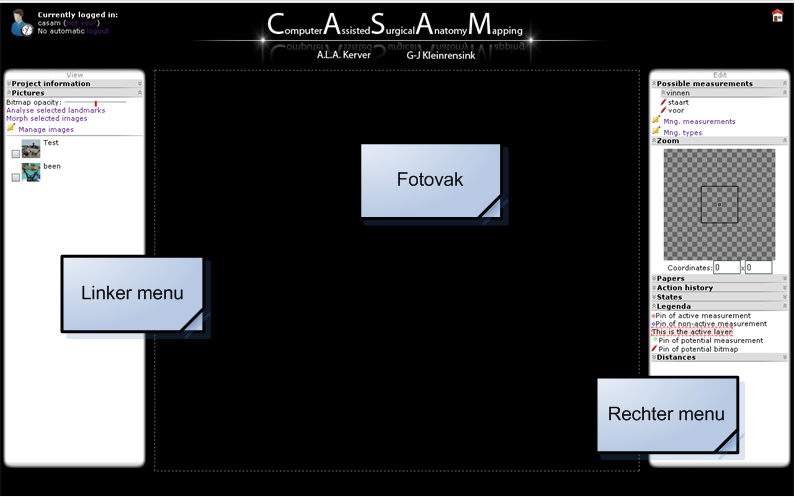
\includegraphics[width=\textwidth]{fig_main}
\caption{De indeling van het hoofdscherm}
\label{fig:hoofdscherm_indeling}
\end{figure}
\\
Wij hebben gekozen voor een indeling met een linker- en rechtermenu met daartussen een gebied waar foto's getoond worden. De beide menu's zijn ingedeeld als gebieden waarin verschillende tabbladen geladen kunnen worden. Omdat niet elk tabblad altijd nodig is, is het mogelijk deze dicht te klappen.
\\
\\
In het linkermenu worden algemene projectgerelateerde instellingen getoond met daaronder de lijst met aan het project gekoppelde foto's met bijbehorende bitmaps en landmarks. In het rechtermenu zijn gereedschappen ondergebracht die bewerkingen met de foto's in het linker menu kunnen doen of hierbij hulp bieden. Bovenin bevindt zich een tabblad waar mogelijke metingen aangemaakt en toegepast kunnen worden op de actieve foto. Daaronder bevinden zich tabbladen waarin wijzigingen ongedaan gemaakt kunnen worden en waarin een ingezoomd deel van de foto bekeken kan worden.
\\
\\
De interface is verder voorzien van een aantal pop-ups waarin enkele objecten beheerd kunnen worden. Er is een scherm waarin foto's toegevoegd en verwijdert kunnen worden, en ook de Mogelijke Metingen en types voor Mogelijke Metingen hebben een eigen pop-up venster. Als de pop-up vensters actief zijn moeten deze eerst gesloten worden voordat verder gewerkt kan worden in het overzicht.
\\
\\
Om de interactie behalve effici\"{e}nt ook mooi te laten verlopen zijn er wat visuele effecten aan toegevoegd. Hierbij hebben we gebruik gemaakt van effecten die Scriptaculous biedt, zoals het oprollen van tabbladen, het laten in- en uitvagen van nieuwe pop-ups op een zwarte achtergrond, etc. Toegevoegde landmarks worden ook even geel gekleurd in het linker menu om aan te geven waar ze terecht komen als ze zijn aangemaakt. 
\\
\\
Om projecten te beheren is een soort thuis-pagina gemaakt waarin bestaande projecten gekozen kunnen worden of nieuwe aangemaakt. De kleine afbeelding die getoond wordt per project wisselt om de paar seconde als slideshow en toont alle foto's die gekoppeld zijn aan het project.

\begin{figure}[htbp]
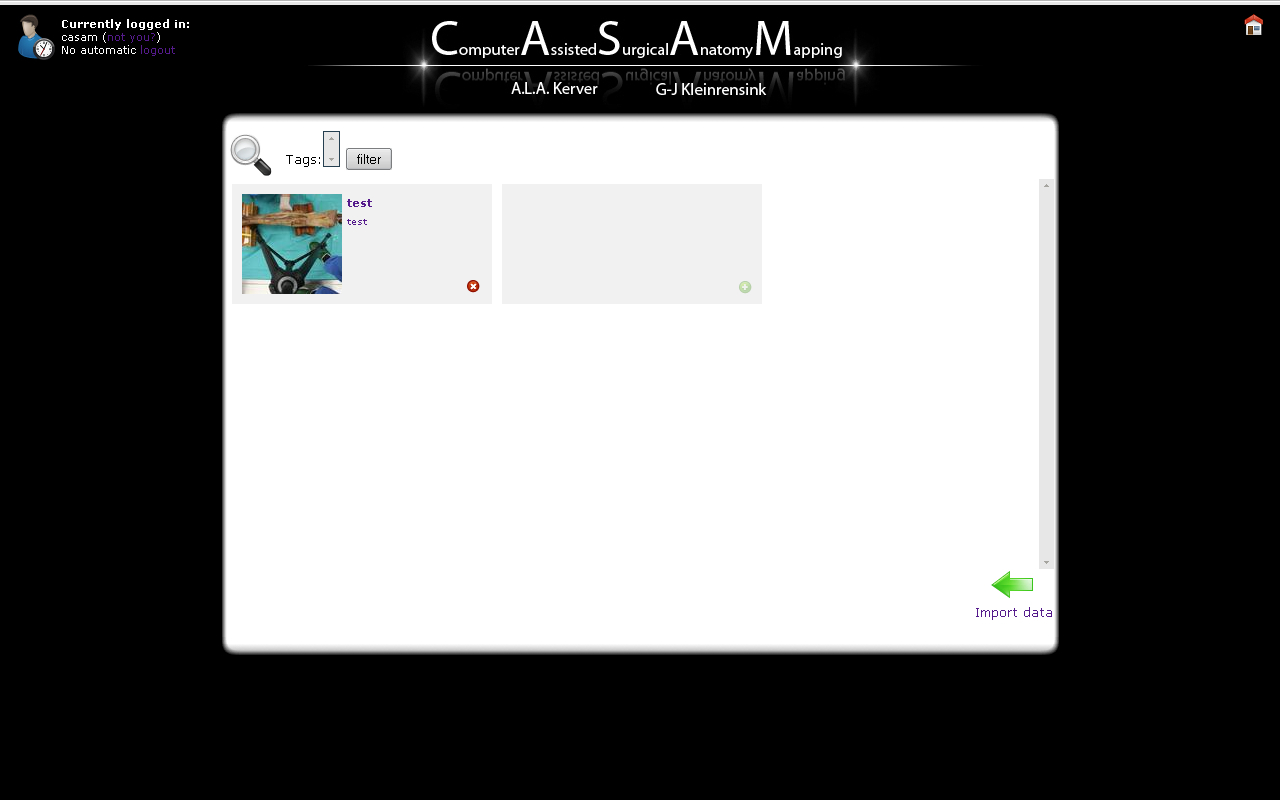
\includegraphics[width=\textwidth]{fig_home}
\caption{De projectselectiepagina}
\label{fig:projectselectiescherm}
\end{figure}

\subsection{Database systeem}
\label{implementatie_database_systeem}
Voordat we konden beginnen met het database systeem, hebben we eerst een database model gemaakt. De eerste versie van dit model is te zien in Figuur \ref{brainstorm_klassediagram}.
De uiteindelijke versie van dit model is te zien in Figuur \ref{databasediagram}.
Een aantal van de belangrijkste wijzgingen zijn:
\begin{description}
  \item[Measurement types] In het originele model was er een algemeen MeasurementType bedacht, waar alle 3 de types van overerven. 
  In het uiteindelijke model was er nog wel ruimte voor MeasurementTypes, maar zijn dit types geworden die aangemaakt kunnen worden door de gebruiker.
  De MeasurementTypes zoals die bedacht waren bestaan uiteindelijk alleen nog uit Measurements en Bitmaps, waarvan Bitmaps overerft vanuit Image, in plaats van een algemeen MeasurementType.
  \item[Measurements] De Measurements zelf zijn nu wat in het originele model een PointMeasurement heette.
  Ook de ProjectMeasurementsList is uit het model verdwenen, en vervangen door de algemene PotentialMeasurements.
  \item[Images] Het algemene type Image is in het uiteindelijke model gespaard gebleven.
  De Pati\"{e}nt die echter aan een OriginalImage hing, is gesneuveld, omdat dit niets toevoegde aan het systeem.
  Ook hebben we besloten om EditedImages niet op te slaan, en in plaats daarvan States te bewaren.
  \item[States en Projectfiles] States zijn samen met de Projectfiles aan het model toegevoegd.
  Hierbij zijn de States bedoeld om de huidige configuratie van zichtbare foto's, Bitmaps en Measurements op te slaan en weer op te halen.
  De Projectfiles zijn bedoeld voor de export van een project.
  \item[Users] In het originele model zou het user-management door Django geregeld worden.
  Tijdens de implementatie is gebleken, dat we toch nog een UserProfile moeten toevoegen.
  In dit UserProfile wordt opgeslagen welke Gebruiker welke rechten heeft op welk project.
\end{description}
Andere aspecten van het database systeem worden hieronder toegelicht.

\subsubsection{Verschillende doorzichtige foto's over elkaar heen leggen om de verschillen te bekijken}
Voor de weergave van afbeeldingen binnen het project is er bedacht dat er meerdere afbeeldingen tegelijk zichtbaar moesten kunnen zijn.
Hiervoor is er vastgesteld dat er verschillende afbeeldingen over elkaar heen gelegd gaan worden, met een door de gebruiker in te stellen volgorde en doorzichtigheid.
Om dit te kunnen realiseren hebben we eerst voor elke afbeelding in het project een eigen slider gemaakt, die pas geladen wordt op het moment dat de afbeelding zichtbaar wordt gemaakt. 
Met deze slider kan de gebruiker vervolgens zelf instellen met welke doorzichtigheid de corresponderende afbeelding zichtbaar gemaakt moet worden.
Deze slider was een onderdeel van de Scriptaculous bibliotheek, waar in het project vaker gebruik van gemaakt is.
\\
\\
Hierna moest het mogelijk gemaakt worden om de volgorde van de weergegeven afbeeldingen aan te passen.
Dit hebben we gedaan door van de lijst met afbeeldingen in het linker frame een Sortable te maken.
Dit heeft als voordeel dat de volgorde nu bepaald kan worden door de gewenste zichtbare afbeelding naar boven te slepen.
Ook wordt de volgorde van de lijst automatisch aangepast op het moment dat er een afbeelding zichtbaar wordt gemaakt, door deze afbeelding naar boven te verplaatsen in de lijst.
De bovenste afbeelding van de lijst wordt altijd ook de bovenste afbeelding van alle zichtbare afbeeldingen, zodat de bovenste afbeelding altijd de actieve afbeelding is, waarop de bewerkingen worden gedaan.

\subsubsection{Herkenningspunten bij de afbeeldingen}
Voor het toevoegen van herkenningspunten aan de afbeeldingen hebben we ervoor gekozen om deze op te slaan in een apart model in de database.
Aan dit model zit een koppeling met de MogelijkeMetingen vast, evenals met de afbeelding waar het punt bij hoort en het project.
Om een herkenningspunt (landmark) op te kunnen slaan, moeten deze eerst bestaan.
Als er een foto geladen is in het scherm, wordt hier met JavaScript een listener aan gekoppeld die reageert als er op de foto geklikt wordt.
Deze listener wordt weer van de foto afgehaald op het moment dat er een andere foto overheen geladen wordt, en er een andere foto bestempeld wordt als actieve laag.
Aan deze foto wordt dan weer een listener gekoppeld, die de muisklik op de foto afvangt.
\\
\\
Als er op de geladen foto's wordt geklikt, wordt de listener (van de foto van de actieve laag) geactiveerd en wordt er een popup-schermpje getoond waarin de benodigde informatie voor het landmark staat.
In deze popup dient er een MogelijkeMeting gekozen te worden van het landmark, en wordt er onzichtbaar een ID meegegeven van de foto.
Als er in de popup dan op 'Save' geklikt wordt, wordt er eerst in de JavaScript code gekeken of het landmark al bestaat of niet.
Voor een landmark dat al bestaat, wordt er een 'repositioning'-change aangemaakt, waarin de nieuwe co\"{o}rdinaten worden opgeslagen, terwijl er voor een nieuw landmark een 'positioning'-change wordt aangemaakt.
Hierna wordt er een AJaX call naar de server gedaan.
Op de server wordt er vervolgens gekeken of er al een landmark bestaat, met het gegeven foto-ID en de gegeven MogelijkeMeting.
Is dit zo, dan wordt dit landmark opgehaald, en aangepast.
Bestaat er nog geen landmark met de gegeven parameters, dan wordt er een nieuwe aangemaakt.
In beide gevallen wordt het bewuste landmark vanuit de database terug gegeven naar JavaScript, door middel van een JSON-string.
Als het landmark opgeslagen kon worden op de server, wordt de hiervoor aangemaakte change in JavaScript ook opgeslagen.
Vervolgens wordt voor een bestaand landmark de positie aangepast.
Voor een bestaand landmark wordt er een nieuw measurement aangemaakt, dat op de goede plaats onder de afbeelding wordt geplaatst.

\subsubsection{Afbeeldingen tekenen over foto's om belangrijke gebieden aan te geven, ook wel bitmaps genoemd}
Een plek in ons systeem waar de samenwerking van verschillende deelsystemen en zelfs verschillende talen goed zichtbaar wordt is de manier waarop de Flash-applicatie gebruikt wordt om bitmaps te tekenen. Hieronder staat dit in een sequence-diagram weergegeven.
\\
\\
Het eerste deel van het diagram toont op welke wijze het bestaan van bitmaps geladen wordt in de JavaScript-omgeving. De rest van het diagram toont wat het systeem doet als de gebruiker het tekenen of bewerken van een bitmap kiest.
\\
\\
Eerst wordt in de HTML-pagina een object ingevoegd waarin de Flash-applicatie geladen wordt. Vervolgens laadt de Flash-applicatie de afbeelding waar op getekend gaat worden. Als de gebruiker vervolgens kiest om de bitmap op te slaan wordt de tekening naar de server verzonden, en als deze succesvol opgeslagen is krijgt de Flash-applicatie een bevestiging waarop deze een melding naar de JavaScript-omgeving gemaakt wordt met het verzoek de Flash-applicatie te sluiten. Dit is de laatste actie die in het diagram beschreven wordt.

\begin{figure}[htbp]
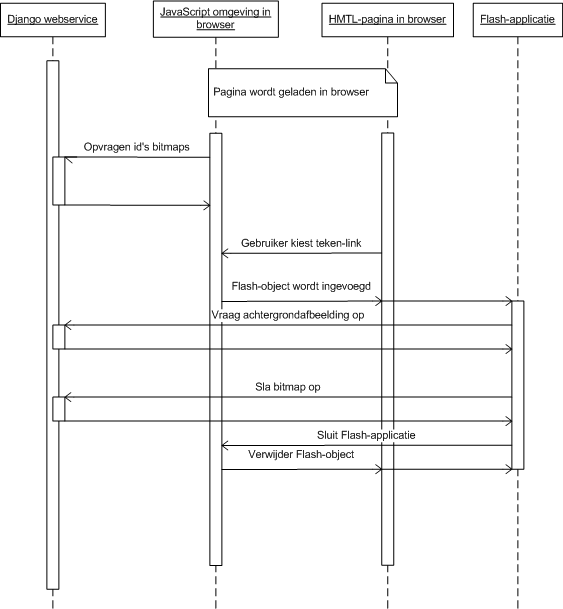
\includegraphics[width=\textwidth]{sequencediagram}
\caption{Sequencediagram}
\label{fig:sequencediagram}
\end{figure}


\subsubsection{Toevoegen van relevante papers en websites}
Voor het toevoegen van papers en websites aan een project hebben wij gekozen om deze ook in een apart model in de database op te slaan.
In dit model zit een verwijzing naar het project waar de toevoeging bij hoort en een verwijzing naar de toevoeging zelf.
Deze verwijzing bestaat in het geval van een website uit een URL, en in het geval van een paper uit een link naar de paper die op de lokale server wordt opgeslagen.

\subsubsection{Tags toevoegen aan projecten om ze te categoriseren}
Om een grote verzameling projecten overzichtelijk te houden was het noodzakelijk om een aantal trefwoorden (tags) aan een project te koppelen.
Ook moest het mogelijk zijn om onderlinge verbanden tussen projecten te leggen door middel van dezelfde tags.
Op deze manier kan er makkelijk gezocht worden op de tags en worden alleen de overeenkomstige projecten getoond.
Bij het aanmaken van een project kan er gekozen worden uit de selectie van bestaande tags, zodat een project direct makkelijk gevonden kan worden.
Voor het aanmaken van nieuwe tags is het wel nodig om het project te openen.
Deze nieuwe tags kunnen daarna direct aan andere projecten worden gekoppeld.

\subsubsection{States}
Een onderdeel dat erg lastig bleek te implementeren waren de states.
States zijn de manier om, wanneer een interessante samenstelling van foto's, landmarks, bitmaps etc. op het scherm staat, deze op te slaan om het later terug te kunnen halen.
Omdat de software voornamelijk was ontworpen om handelingen te verrichten bij interactie van de gebruiker, bleek het erg moeilijk te zijn om via code een eerder opgeslagen state te herstellen.
Om dit mogelijk te maken is een ander HTML en JavaScript model nodig, waarvoor een aanbeveling wordt gedaan in hoofdstuk 7.
Omdat deze aanpassingen nog niet doorgevoerd zijn is een tijdelijke oplossing ge\"{i}mplementeerd die een deel van de HTML structuur opslaat wanneer de gebruiker erom vraagt, en deze kan later in een popup weer worden getoond zodat een soort van statische state ontstaat waar niet in verder gewerkt kan worden.
Een andere manier zou zijn om de state op te slaan in een plaatje, waarbij het renderen van de browser wordt nagebootst door de Python Image Library.
Omdat deze manier een moeilijkere implementatie heeft dan het kopie\"eren van de HTML, en niet per s\'e een beter resultaat oplevert, is ervoor gekozen om dit niet te implementeren.

\subsubsection{Afstanden meten in foto's}
We hebben een spike solutions geschreven voor het meten van afstanden in foto's. 
Mede door tijdsgebrek en de afhankelijkheid van andere spike solutions zijn we er niet aan toegekomen om dit te implementeren. 
In sectie \ref{customjaap} gaan we hier verder op in.

\subsubsection{Exporteren}
Teneinde het uitwisselen van projecten mogelijk te maken is er een export functionaliteit geschreven die de beheerder in staat stelt een project met alle gegevens die daarbij horen te exporteren, en later weer te importeren.
Om de export zo min mogelijk afhankelijk te maken van het systeem is gekozen voor een export naar een zipfile, zodat deze zipfile ook zonder het programma gebruikt kan worden om gegevens terug te halen door deze uit te pakken en het daarin bevatte script handmatig uit te voeren.
In normaal gebruik kan de export opgeslagen worden teneinde op een later tijdstip weer naar het systeem geupload te worden waarna het automatisch geimporteerd wordt.

\subsection{Image Processing}
\label{implementatie_image_processing}
Image Processing was \'{e}\'{e}n van de grootste uitdagingen van het project. 
Niemand had ervaring met de verschillende bibliotheken of uitgebreide ervaring met dit aspect van Image Processing. 
Er waren verschillende opties om de benodigde technieken te implementeren. 
Zo konden we ze zelf implementeren met behulp van Numpy\cite{numpy} of gebruik maken van grotere bibliotheken zoals Insight Segmentation and Registration Toolkit (ITK)\cite{ITK} of de Visualization Toolkit (VTK)\cite{vtk}. 
Verder was er nog de Python Imaging Library (PIL)\cite{pil} die geschikt is om eenvoudige beeldbewerking te doen. 
Uiteindelijk is er, mede op advies van Dr. Botha, gekozen voor PIL in combinatie met de VTK bibliotheek. 
Om aan de vraagstelling te kunnen voldoen, het in kaart brengen van de variaties per landmark en het kunnen projecteren van getekende gebieden op \'{e}\'{e}n gemiddeld plaatje, hebben we gekozen om een deel van de methode Active Shape Modeling, genaamd Point Distribution Models, toe te passen in combinatie met Thin Plate Spline transformaties. 
Hierdoor is het mogelijk voor de onderzoeker om op een wiskundig verantwoorde manier anatomische structuren op een gemiddelde te projecteren en de variaties per landmark te visualiseren.
Al snel bleek dat er veel onderzoek nodig was om de theorie achter Principal Component Analysis, Active Shape Models, Point Distribution Models en de Thin Plate Spline Transformaties te doorgronden. 
Ook kostte het enige extra tijd om met de VTK bibliotheek bekend te raken.

\subsubsection{Point Distribution Model}
Om het Point Distribution Model te maken is een set nodig van verschillende landmarks waarvan de variaties en de gemiddelden interessant zijn om weer te geven. 
Het is van belang om de landmarks zo te kiezen dat ze makkelijk zijn te vinden in elke foto en belangrijke punten aangeven op de structuur waar het om gaat. 
De gebruiker kan landmarks in de foto aangeven door eerst een landmarktype aan te maken, dan een landmark van een bepaald type en hierbij aan te geven of het een shapedefining landmark is of niet. 
Nadat de gebruiker in de foto's de gewenste landmarks heeft aangegeven kan hij door 'Analyse selected landmarks' aan te klikken het Point Distribution Model van de geselecteerde landmarks laten uitrekenen en weergeven.
\\
\begin{figure}[htbp]
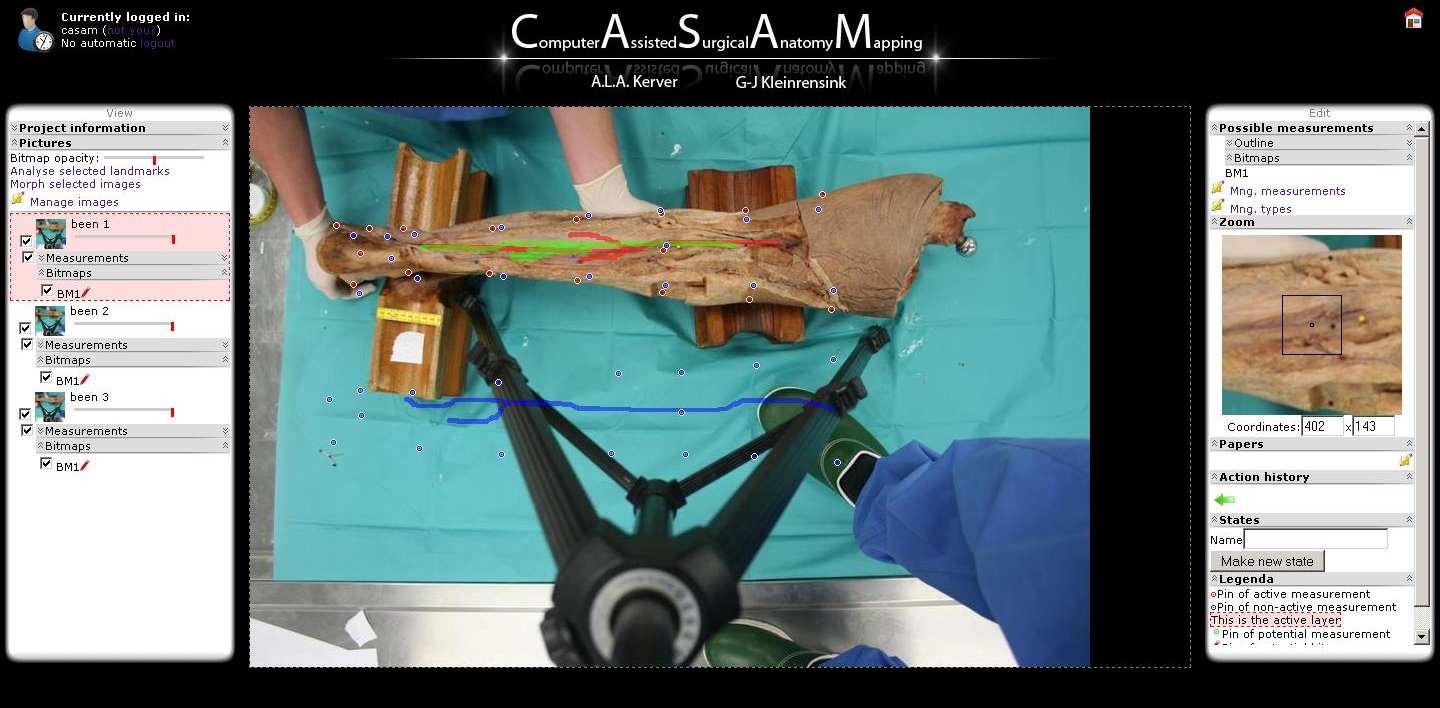
\includegraphics[width=\textwidth]{screen1}
\caption{Drie verschillende benen met hun landmarks en bitmaps}
\label{fig:screen1}
\end{figure}
\\
Op dit moment wordt in JavaScript gecontroleerd welke images en landmarks geselecteerd zijn en wordt er via een AJaX request de id's van de afbeeldingen en de geselecteerde landmarks per afbeelding doorgegeven. 
Aan de hand van de id's van de afbeelding en de landmarks worden vervolgens de bijbehorende objecten uit de database gehaald. 
In de view wordt getest of de geselecteerde landmarks wel geschikt zijn om een Point Distribution Model van te maken. 
Dit is bijvoorbeeld niet zo als: er geen landmarks geselecteerd zijn, er te weinig landmarks geselecteerd zijn van een type of de geselecteerde landmarks van een geheel ander type zijn. 
In elk van deze gevallen wordt er een foutmelding aan de gebruiker gegeven in de vorm van een JavaScript alert met de aard van de fout, zodat de gebruiker zijn selectie kan aanpassen.
\\
\\
Als de juiste landmarks zijn geselecteerd wordt er allereerst via de co\"{o}rdinaten van de landmarks per afbeelding een vtkUnstructuredGrid aangemaakt met de desbetreffende punten erin als vertices. 
Vervolgens wordt over deze grids de Generalized Procrustes Analysis uitgevoerd via het vtkProcrustesAlignmentFilter. 
Dit zorgt ervoor dat de gevonden modi van variatie onafhankelijk van de positie en de rotatie van de objecten zijn. 
Door ervoor te kiezen om de mode op RigidBody te zetten blijft echter wel de grootte van de structuren behouden. 
De opgeslagen grids zijn nu iteratief getransleerd en geroteerd naar elkaar toe.
\\
\\
Nu is het tijd om de Principal Component Analysis (PCA) op de aligned grids uit te voeren, dit is gedaan met behulp van het vtkPCAAnalysisFilter.
Uit het resultaat kunnen de gemiddelde posities per landmark gehaald worden. 
We hebben er voor gekozen om de eerste twee modi van variatie te berekenen, de hoofdmodus van variatie (eerste mode) zorgt altijd voor de grootste verandering en is de eigenvector met de grootste eigenwaarde die uit de PCA komt. 
Om deze variaties te berekenen vragen we de GetParameterisedShape en berekenen we hiermee voor de eerste en tweede modus de extremen, dit zijn plus en min 3 standaarddeviaties van het gemiddelde.
\\
\begin{figure}[htbp]
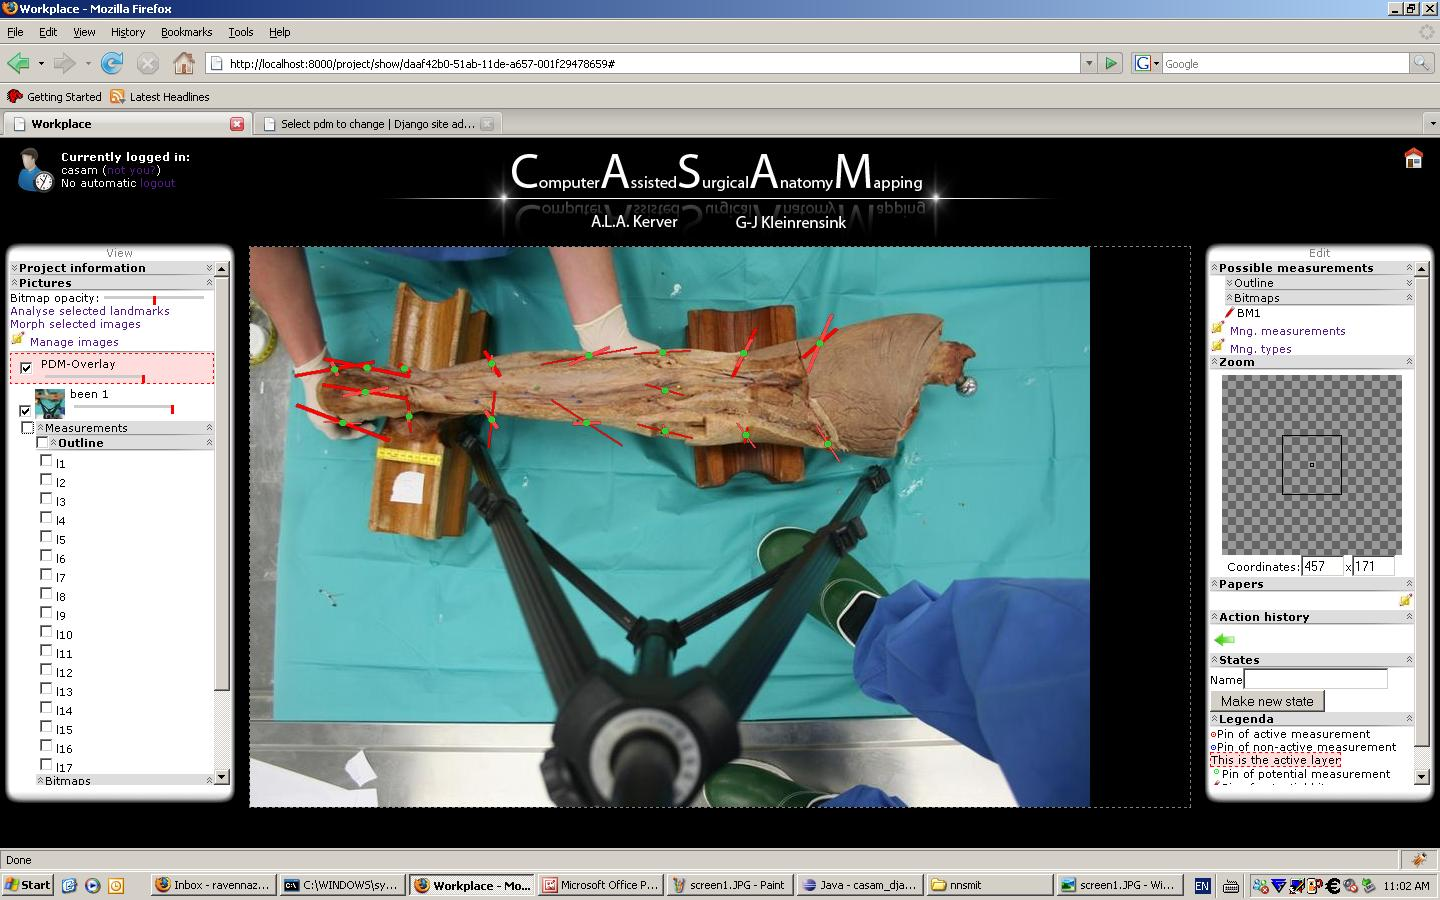
\includegraphics[width=\textwidth]{screen2}
\caption{Point Distribution Model van de outlines van 3 benen}
\label{fig:screen2}
\end{figure}
\\
Nu we de benodigde co\"{o}rdinaten hebben (gemiddelden en extremen) kunnen we beginnen aan de visualisatie van de landmarks. 
Dit wordt gedaan met behulp van de PIL. Aan de hand van de afmetingen van de originele foto's en de gegeven co\"{o}rdinaten wordt voor het gemiddelde een ellips getekend. 
Tussen de extremen van de twee hoofdmodi van variatie wordt een lijn getekend. 
De lengte van deze lijn geeft de grootte van de mogelijke variatie aan op basis van de voorbeelden uit de gegeven landmarks. 
Door de ellipsoids en lijnen weer te geven met een doorzichtige achtergrond is het vervolgens mogelijk om deze als een overlay over de images te projecteren. 
De overlay wordt opgeslagen in de database en is beschikbaar voor weergave vanuit de interface.

\subsubsection{Thin Plate Spline Transformatie}
Om de daadwerkelijke morph uit te voeren van de getekende structuren moesten we eerst een transformatie uitvoeren om verschillen in translaties en rotaties tussen de verschillende foto's te verwijderen. 
Na overleg met dr. Botha is besloten om dit niet via Generalized Procrustes Aligment te doen, maar om \'{e}\'{e}n foto (in dit geval de eerste) als voorbeeld te nemen en alle andere getekende structuren naar deze foto te morphen. 
Hierdoor ontstaat een foto met een bestaande anatomie. Dit heeft een groot voordeel ten op zichte van het morphen van alle foto's naar een gemiddelde, want dan onstaat er een gemiddelde foto zonder bestaande anatomie. 
Helaas kwam de implementatie van dit onderdeel van het project te laat om ook nog het Point Distribution Model volgens deze gedachte te implementeren. 
\\
\\
In grote lijnen werkt de implementatie op dezelfde manier als die van het Point Distribution Model met een paar verschillen. 
Wederom worden landmarks uit de interface ingelezen en opgehaald. 
Er wordt naast de eerdergenoemde checks ook nog gekeken of de landmarks wel allemaal shapedefining zijn. 
Voor het morphproces worden namelijk een ander soort landmarks gebruikt dan voor het berekenen van het Point Distribution Model. 
De shapedefining landmarks zijn landmarks die kenmerkend zijn voor de vorm van het hele object (je kunt bijvoorbeeld denken aan de bony landmarks van het been met daartussen op gelijke afstanden geplaatste landmarks op de omtrek van het been). 
\\
\\
Met de gevonden foto's en de bijbehorende landmarks worden de co\"{o}rdinaten van de landmarks ditmaal direct in vtkPoints objecten gezet. 
Deze vtkPoints worden gebruikt in de vtkLandmarkTransform. 
Als source landmarks worden per foto de vtkPoints gebruikt en als target de vtkPoints van het gekozen active image. 
Via vtkImageReslice wordt de daadwerkelijke transformatie uitgevoerd. 
We kiezen Nearest Neighbour als interpolationmode om ervoor te zorgen dat de kwaliteit van de getekende structuren niet verslechtert. 
Net als bij het Point Distribution Model wordt de mode op RigidBody gezet om informatie over de grootte niet te verliezen. 
Vervolgens wordt de output van deze transformatie gebruikt als source voor de daadwerkelijke morph. 
Het morphen zelf wordt ge\"{i}mplementeerd met behulp van de vtkThinPlateSplineTransform. 
De source landmarks zijn gelijk aan de output van de eerste transformatie, voor de target landmarks zijn weer de landmarks van het gekozen active image gekozen. 
Via de vtkImageReslice wordt nu het eindresultaat bereikt, de bitmaps van alle geselecteerde foto's worden nu, gemorpht naar de active image, weergegeven.


\subsubsection{Tekenen}
Vanuit de applicatie kan op twee manieren de Flash-applicatie gestart worden. 
Het kan door in het rechter scherm met Possible Measurements een nieuwe bitmap aan te maken terwijl een afbeelding actief is. 
De tweede methode is om een bestaande bitmap die aan een image gekoppeld is te bewerken door in het linker vak op de edit-knop te klikken.
\\
\\
Dit opent de Flash-applicatie waaraan in een HTML-tag argumenten meegegeven worden, zoals een verwijzing naar de achtergrondfoto en optioneel een bestaande bitmap. 
In de Flash-applicatie kan vervolgens in een aparte laag getekend worden in \'{e}\'{e}n kleur. 
Als op de Save-knop gedrukt wordt scant de Flash-applicatie de hele tekenlaag per pixel om een compacte representatie te maken van de tekening. Deze wordt vervolgens naar de server gestuurd met een HTTP-POST, samen met andere gegevens. 
Als de server dit succesvol afvangt en verwerkt krijgt de Flash-applicatie een antwoord en roept de applicatie een JavaScript-functie in de browser aan die de Flash-applicatie afsluit.
\\
\\
Een probleem dat optrad bij grote foto's was dat het afscannen van de tekenlaag enkele seconden kon duren. 
Om deze reden is er een extra optimalisatie ingebouwd: de applicatie houdt bij in welk gebied getekend is door een minimale en maximale x en y bij te houden. 
Op deze manier hoeft maar een beperkt deel van de laag gescand te worden, wat meestal significant veel tijd bespaard. 
In het ergste geval is over de hele foto getekend en dan levert deze optimalisatie geen winst maar ook geen verlies op. 
Omdat de applicatie bij elke muisbeweging wel de minimale en maximale co\"{o}rdinaten bijwerkt kan het zijn dat zij iets minder gevoelig is voor de tekenbeweging zelf, maar uit tests bleek dat dit niet storend was.
\\
\\
Als een al bestaande bitmap wordt geladen worden daarbij ook de vorige minimale en maximale co�rdinaten geladen. 
Binnen dat bereik scant de Flash-applicatie de oude bitmap pixel voor pixel af totdat de eerste gekleurde pixel gevonden wordt om de vorige kleur te pakken te krijgen. 

\subsubsection{Tekenen: de serverkant}
De POST van de Flash-applicatie is zo compact mogelijk opgebouwd. 
Deze bestaat uit een header met de afmetingen en de co\"{o}rdinaten van het tekengebied. 
De data zelf bestaan uit nummers die aangeven hoeveel pixels aaneengesloten gekleurd zijn of niet. 
Op deze manier bestaat dus een compleet gekleurde bitmap maar uit \'{e}\'{e}n getal.
\\
\\
De server bouwt deze representatie om naar een grote string met \'{e}\'{e}n karakter per pixel, die met een methode uit de PIL opgeslagen kan worden als GIF-afbeelding. 
Er wordt ook een palet gekoppeld aan de GIF-afbeeldingen met als 255'ste waarde de kleur die in de Flash-applicatie gekozen is. 
Op deze manier wordt de bitmap die in de Flash-applicatie nog uit meerdere kleuren kon bestaan opgeslagen als een GIF-afbeelding met de laatst gebruikte kleur.
